\documentclass{article}

\usepackage[english]{babel}

\usepackage[letterpaper,top=2cm,bottom=2cm,left=3cm,right=3cm,marginparwidth=1.75cm]{geometry}

% Useful packages
\usepackage{amsmath}
\usepackage{graphicx}
\usepackage[table,xcdraw]{xcolor}
\usepackage[colorlinks=true, allcolors=blue]{hyperref}

\begin{document}

\begin{titlepage}
\begin{center}
   \vspace{5cm}
       \large
       \textbf{Steal a Car! Project}\break\break
        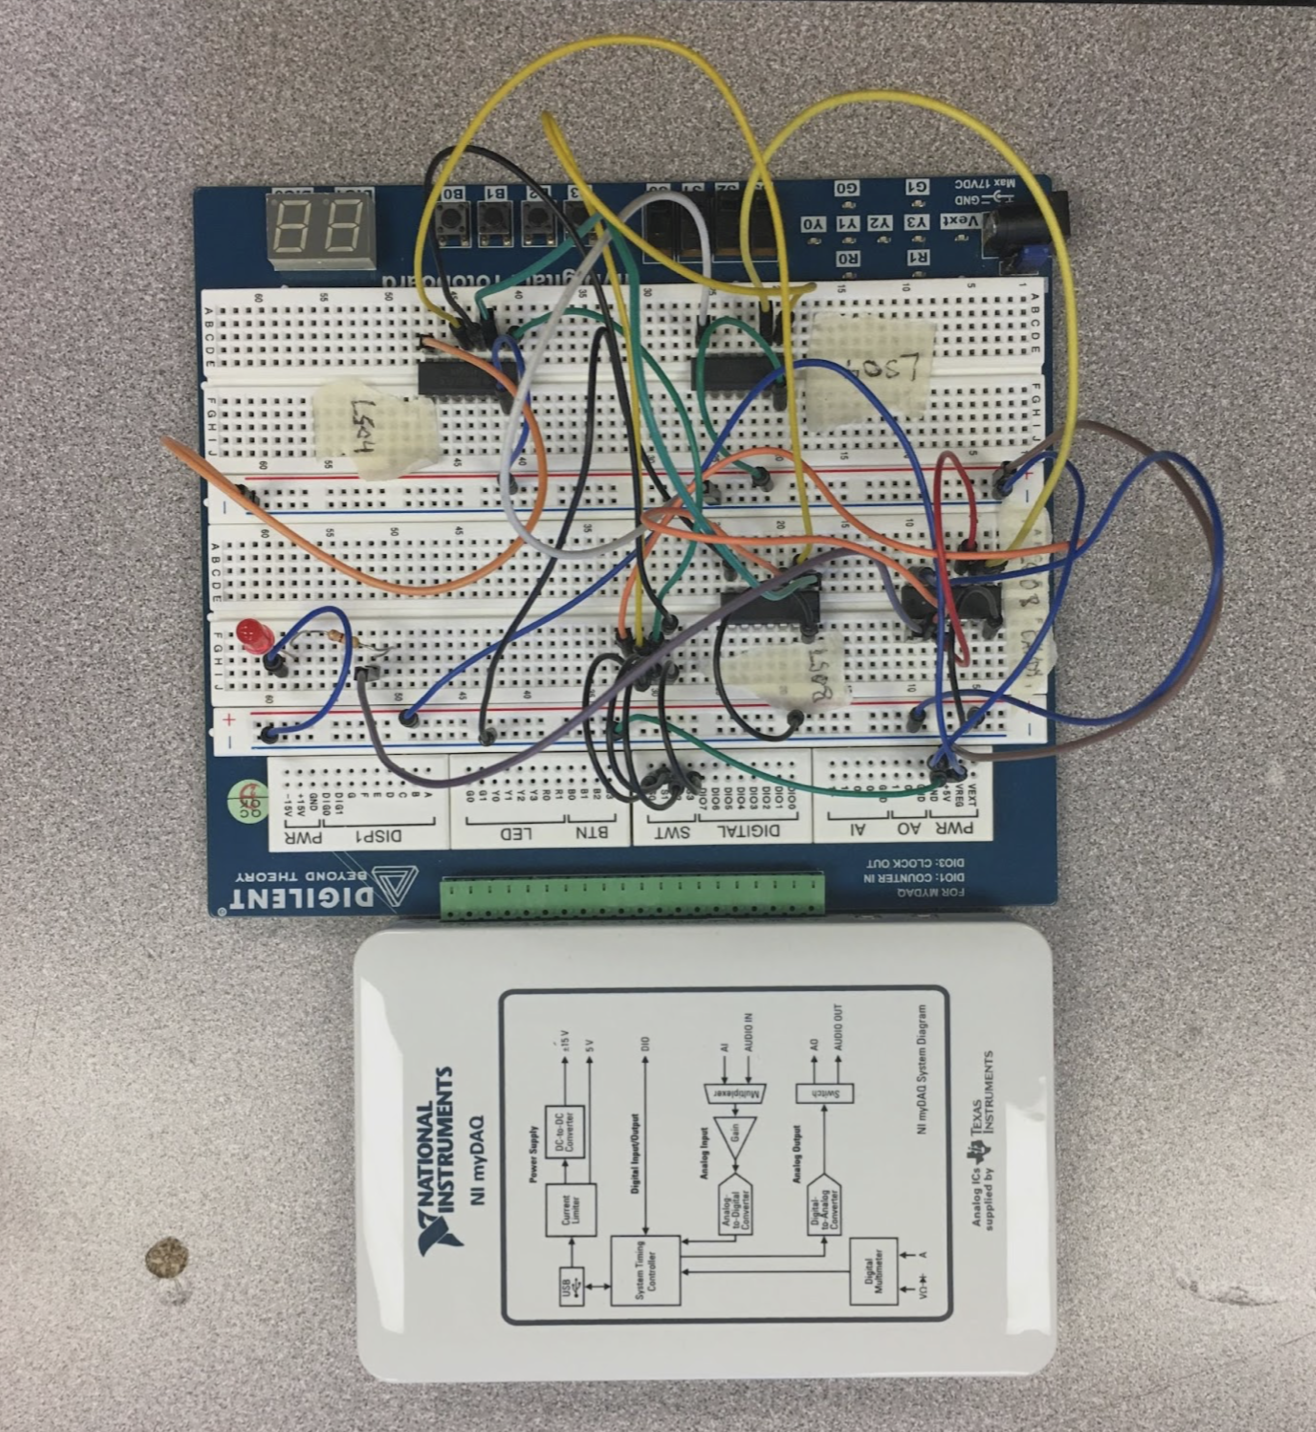
\includegraphics[width=0.9\textwidth]{circuit.png}\break\break
        \text{Damita Sara George \& Ella Xu}\break
        \text{Honors Digital Electronics}\break
        \text{Period 5}\break
        \text\today\break
    \end{center}
\end{titlepage}

\title{Steal a Car! Project}
\tableofcontents

\newpage

\section{Abstract}

The goal of the ‘Steal A Car’ project was to build a circuit using logic gates in a way that only one combination of inputs would successfully turn on a red LED, starting the “engine” of the car. Any other combination would have an output of zero, having no effect on the circuit. Making the combination more complicated with complex logic expressions would make the car more secure, and more difficult to break into. The second part of the project involved taking another group’s circuit and reverse engineering it to successfully find their combination and break into their car. We did this by observing the path of the wires in the other group’s circuit, drawing out the logic, and writing out the truth table logic for the circuit.

\section{Planning}

\subsection{Logic Circuit}

\begin{figure}[!htb]
\centering
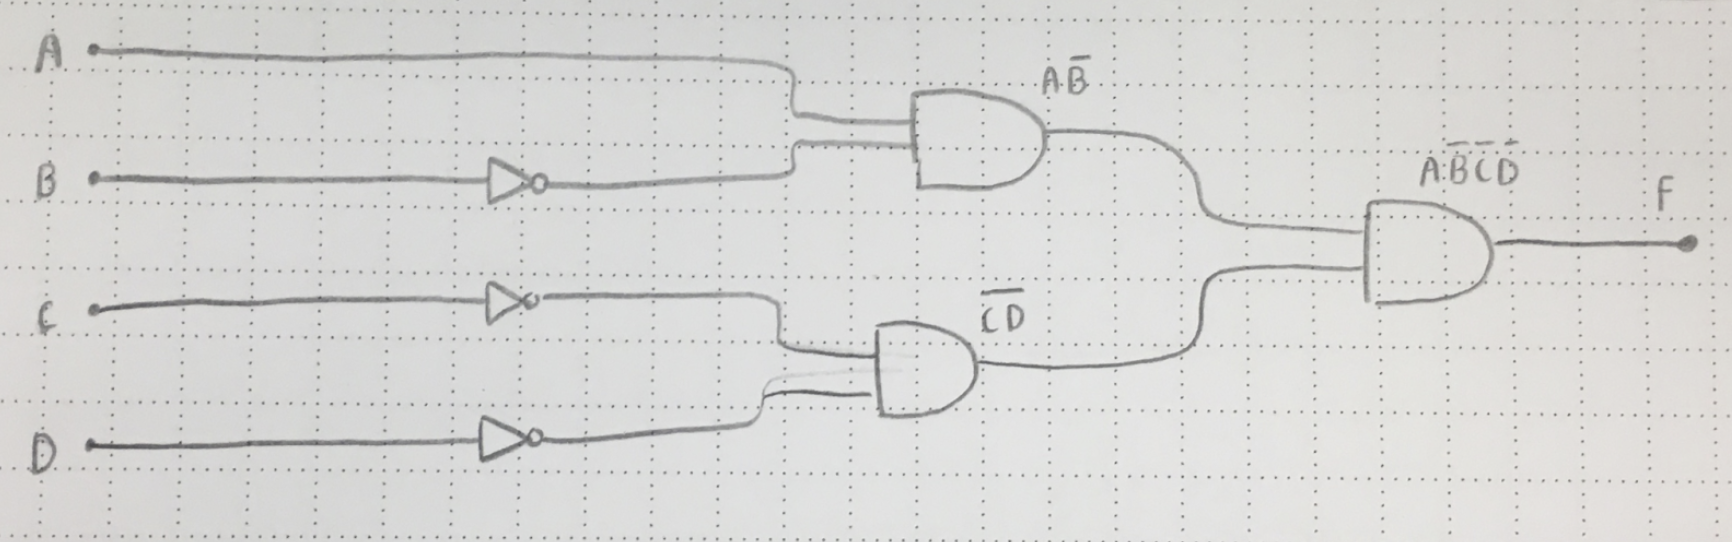
\includegraphics[width=0.6\textwidth]{logic.png}
\caption{\label{fig:logic}This is the series of logic gates we designed.}
\end{figure}

\subsection{Truth Table \& Logic Expression}

\begin{table}[!htb]
\centering
\begin{tabular}{c|c|c|c|c}
{\color[HTML]{000000} A = S0} & {\color[HTML]{000000} B = S1} & {\color[HTML]{000000} C = S2} & {\color[HTML]{000000} D = S3} & {\color[HTML]{000000} F} \\
{\color[HTML]{000000} 0}      & {\color[HTML]{000000} 0}      & {\color[HTML]{000000} 0}      & {\color[HTML]{000000} 0}      & {\color[HTML]{000000} 0} \\
{\color[HTML]{000000} 0}      & {\color[HTML]{000000} 0}      & {\color[HTML]{000000} 0}      & {\color[HTML]{000000} 1}      & {\color[HTML]{000000} 0} \\
{\color[HTML]{000000} 0}      & {\color[HTML]{000000} 0}      & {\color[HTML]{000000} 1}      & {\color[HTML]{000000} 0}      & {\color[HTML]{000000} 0} \\
{\color[HTML]{000000} 0}      & {\color[HTML]{000000} 0}      & {\color[HTML]{000000} 1}      & {\color[HTML]{000000} 1}      & {\color[HTML]{000000} 0} \\
{\color[HTML]{000000} 0}      & {\color[HTML]{000000} 1}      & {\color[HTML]{000000} 0}      & {\color[HTML]{000000} 0}      & {\color[HTML]{000000} 0} \\
{\color[HTML]{000000} 0}      & {\color[HTML]{000000} 1}      & {\color[HTML]{000000} 0}      & {\color[HTML]{000000} 1}      & {\color[HTML]{000000} 0} \\
{\color[HTML]{000000} 0}      & {\color[HTML]{000000} 1}      & {\color[HTML]{000000} 1}      & {\color[HTML]{000000} 0}      & {\color[HTML]{000000} 0} \\
{\color[HTML]{000000} 0}      & {\color[HTML]{000000} 1}      & {\color[HTML]{000000} 1}      & {\color[HTML]{000000} 1}      & {\color[HTML]{000000} 0} \\
{\color[HTML]{000000} 1}      & {\color[HTML]{000000} 0}      & {\color[HTML]{000000} 0}      & {\color[HTML]{000000} 0}      & {\color[HTML]{000000} 1} \\
{\color[HTML]{000000} 1}      & {\color[HTML]{000000} 0}      & {\color[HTML]{000000} 0}      & {\color[HTML]{000000} 1}      & {\color[HTML]{000000} 0} \\
{\color[HTML]{000000} 1}      & {\color[HTML]{000000} 0}      & {\color[HTML]{000000} 1}      & {\color[HTML]{000000} 0}      & {\color[HTML]{000000} 0} \\
{\color[HTML]{000000} 1}      & {\color[HTML]{000000} 0}      & {\color[HTML]{000000} 1}      & {\color[HTML]{000000} 1}      & {\color[HTML]{000000} 0} \\
{\color[HTML]{000000} 1}      & {\color[HTML]{000000} 1}      & {\color[HTML]{000000} 0}      & {\color[HTML]{000000} 0}      & {\color[HTML]{000000} 0} \\
{\color[HTML]{000000} 1}      & {\color[HTML]{000000} 1}      & {\color[HTML]{000000} 0}      & {\color[HTML]{000000} 1}      & {\color[HTML]{000000} 0} \\
{\color[HTML]{000000} 1}      & {\color[HTML]{000000} 1}      & {\color[HTML]{000000} 1}      & {\color[HTML]{000000} 0}      & {\color[HTML]{000000} 0} \\
{\color[HTML]{000000} 1}      & {\color[HTML]{000000} 1}      & {\color[HTML]{000000} 1}      & {\color[HTML]{000000} 1}      & {\color[HTML]{000000} 0}
\end{tabular}
\caption{\label{fig:truth table}This is the truth table that represents the various possible outcomes of the logic circuit.}
\end{table}
\newpage
\subsection{Schematic}

\begin{figure}[!htb]
\centering
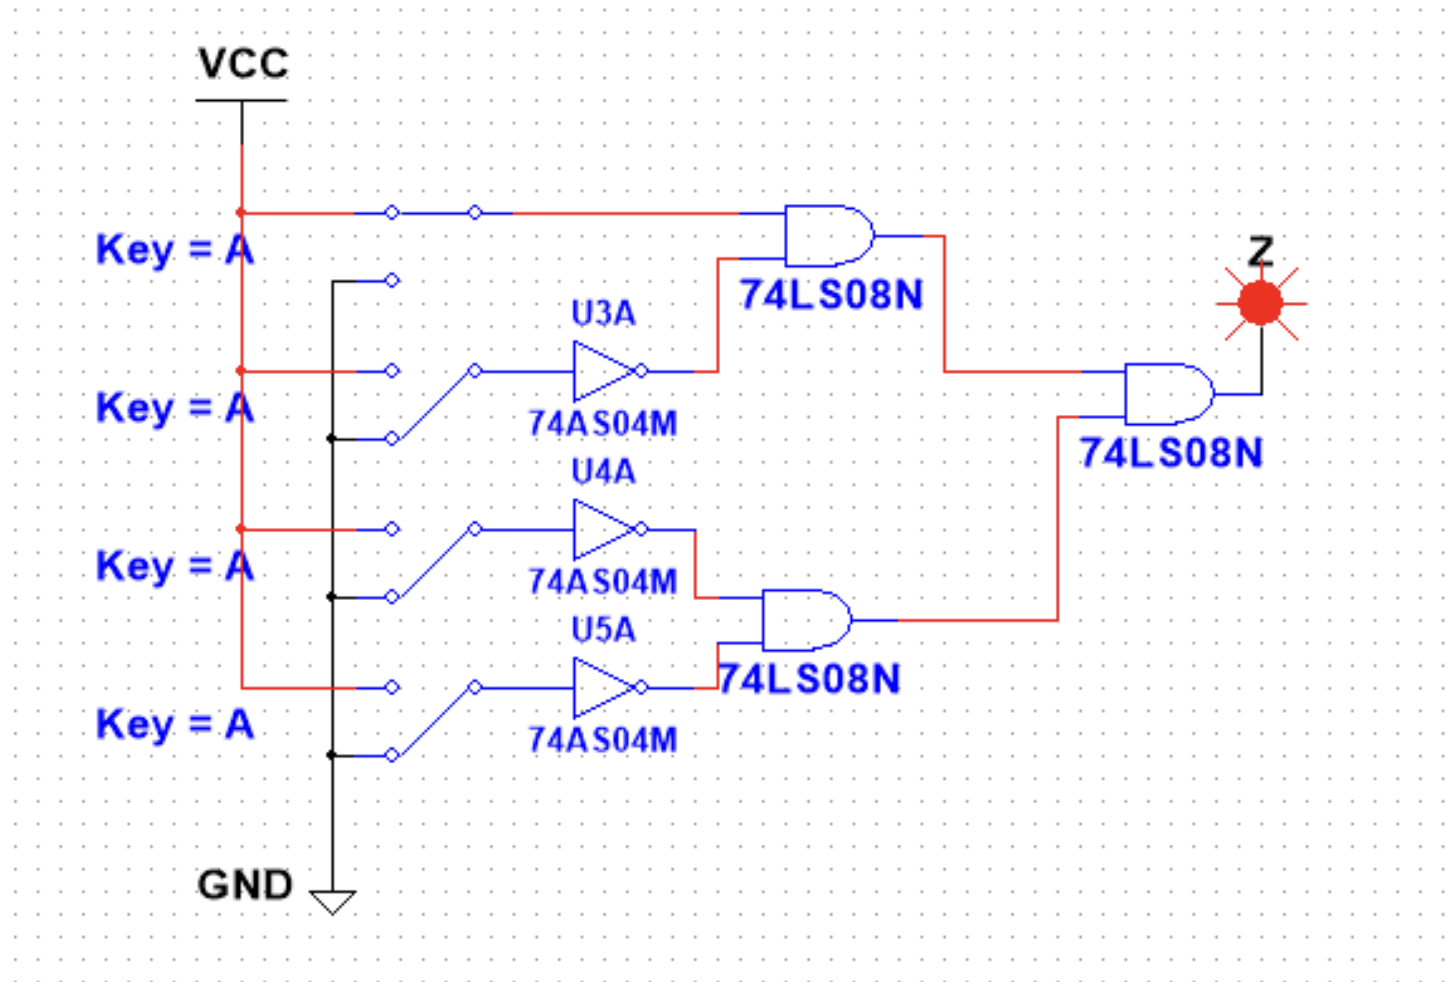
\includegraphics[width=0.6\textwidth]{schematic.png}
\caption{\label{fig:schematic}This is the schematic of the logic circuit, designed in NI Multisim.}
\end{figure}

\section{Build Process}

The first step of the build process was to determine the boolean logic equation and create the truth table. Then, we created a schematic of the logic circuit in Multisim. During this process, we ensured that the logic gates only had one combination that would return the boolean value of one, while all other combinations would return zero. Using the circuit as designed in the Multisim, we selected ICs that would give us three two-input AND gates and three INV gates. To add complexity, we used multiple ICs to increase the amount of wires going across the breadboard. We ended up using two LS08 AND chips and two LS04 INV (inverter) chips.
	
We encountered a problem in our build process when our circuit did not work when we initially tested it out. To solve this issue, we had to troubleshoot the circuit and individually examine each wire leading into the gates and the LED and we eventually found one wire that was not correctly lined up with the rest of the circuit. After adjusting the wire and making sure that the circuit was closed correctly, our LED turned on with the correct combination of switches. 

\section{Conclusion}

This project was beneficial as it allowed us to both build and reverse-engineer circuits. We could work with logic expressions in a more abstract manner, such as when we initially brainstormed our logic expression and truth table, and in a concrete manner, when we actually built our circuit and had the opportunity to examine another circuit.

It also taught us to troubleshoot effectively, as making the best use of our time when we identified mistakes was essential to completing the project within our planned time limit.

\end{document}